\chapter{Appendix}
\label{AppendixA}

\section{Emission Scopes}
\label{sec:emission_scopes}
The thesis will assume familiarity with the concept of Scopes 1, 2, and 3 emissions which I am going to introduce in this section. In carbon-accounting and emissions reporting, it is very important to distinguish between three types of emissions: Scope 1, Scope 2, and Scope 3 emissions  \cite{Bernoville2022Scopes}. Each category represents a different level of emissions associated with an organization's activities as shown in Figure \ref{fig:emission_scopes}.

\begin{itemize}
    \item \textbf{Scope 1} emissions are direct emissions from owned or controlled sources. This includes emissions from company vehicles, and emissions from chemical processes or combustion in owned or controlled boilers, furnaces, etc.
    \item \textbf{Scope 2} emissions are indirect emissions from the generation of purchased electricity, steam, heating, and cooling consumed by the reporting company. These emissions occur at the facility where the energy is generated, not at the point of consumption.
    \item \textbf{Scope 3} emissions are all indirect emissions (not included in Scope 2) that occur in the value chain of the reporting company. This includes both upstream and downstream emissions, encompassing a wide range of activities such as the extraction and production of purchased materials, transportation of purchased fuels, and use of sold products and services.
\end{itemize}

\begin{figure}[h]
    \centering
    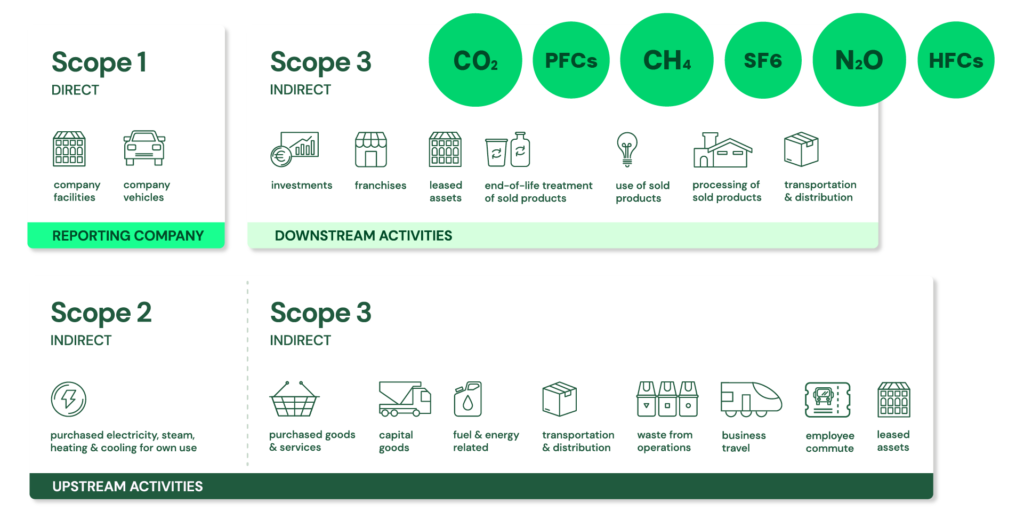
\includegraphics[width=1\textwidth]{figures/emission_scopes.png}
    \caption{Emissions Scopes 1, 2, and 3 . Adapted from \cite{Bernoville2022Scopes}.}
    \label{fig:emission_scopes}
\end{figure}

\section{Marginal Abatement Cost Curve}
\label{sec:MACC}

A Marginal Abatement Cost Curve (MACC) is a graphical representation of the cost of reducing GhG emissions. It is a tool used to identify the most cost-effective measures to reduce emissions. The MACC is a plot of the cost of abating one additional unit of emissions against the quantity of emissions abated. The curve is typically upward-sloping, indicating that the cost of abating additional emissions increases as more emissions are reduced. The MACC is a useful tool for policymakers and businesses to identify the most cost-effective measures to reduce emissions \cite{McKinsey2017}. It can also be used to compare the cost-effectiveness of different emission reduction measures and to identify the most cost-effective measures to achieve a set emissions reduction target. Figure~\ref{fig:macc} shows an example of a MACC.

\begin{figure}[H]
\centering
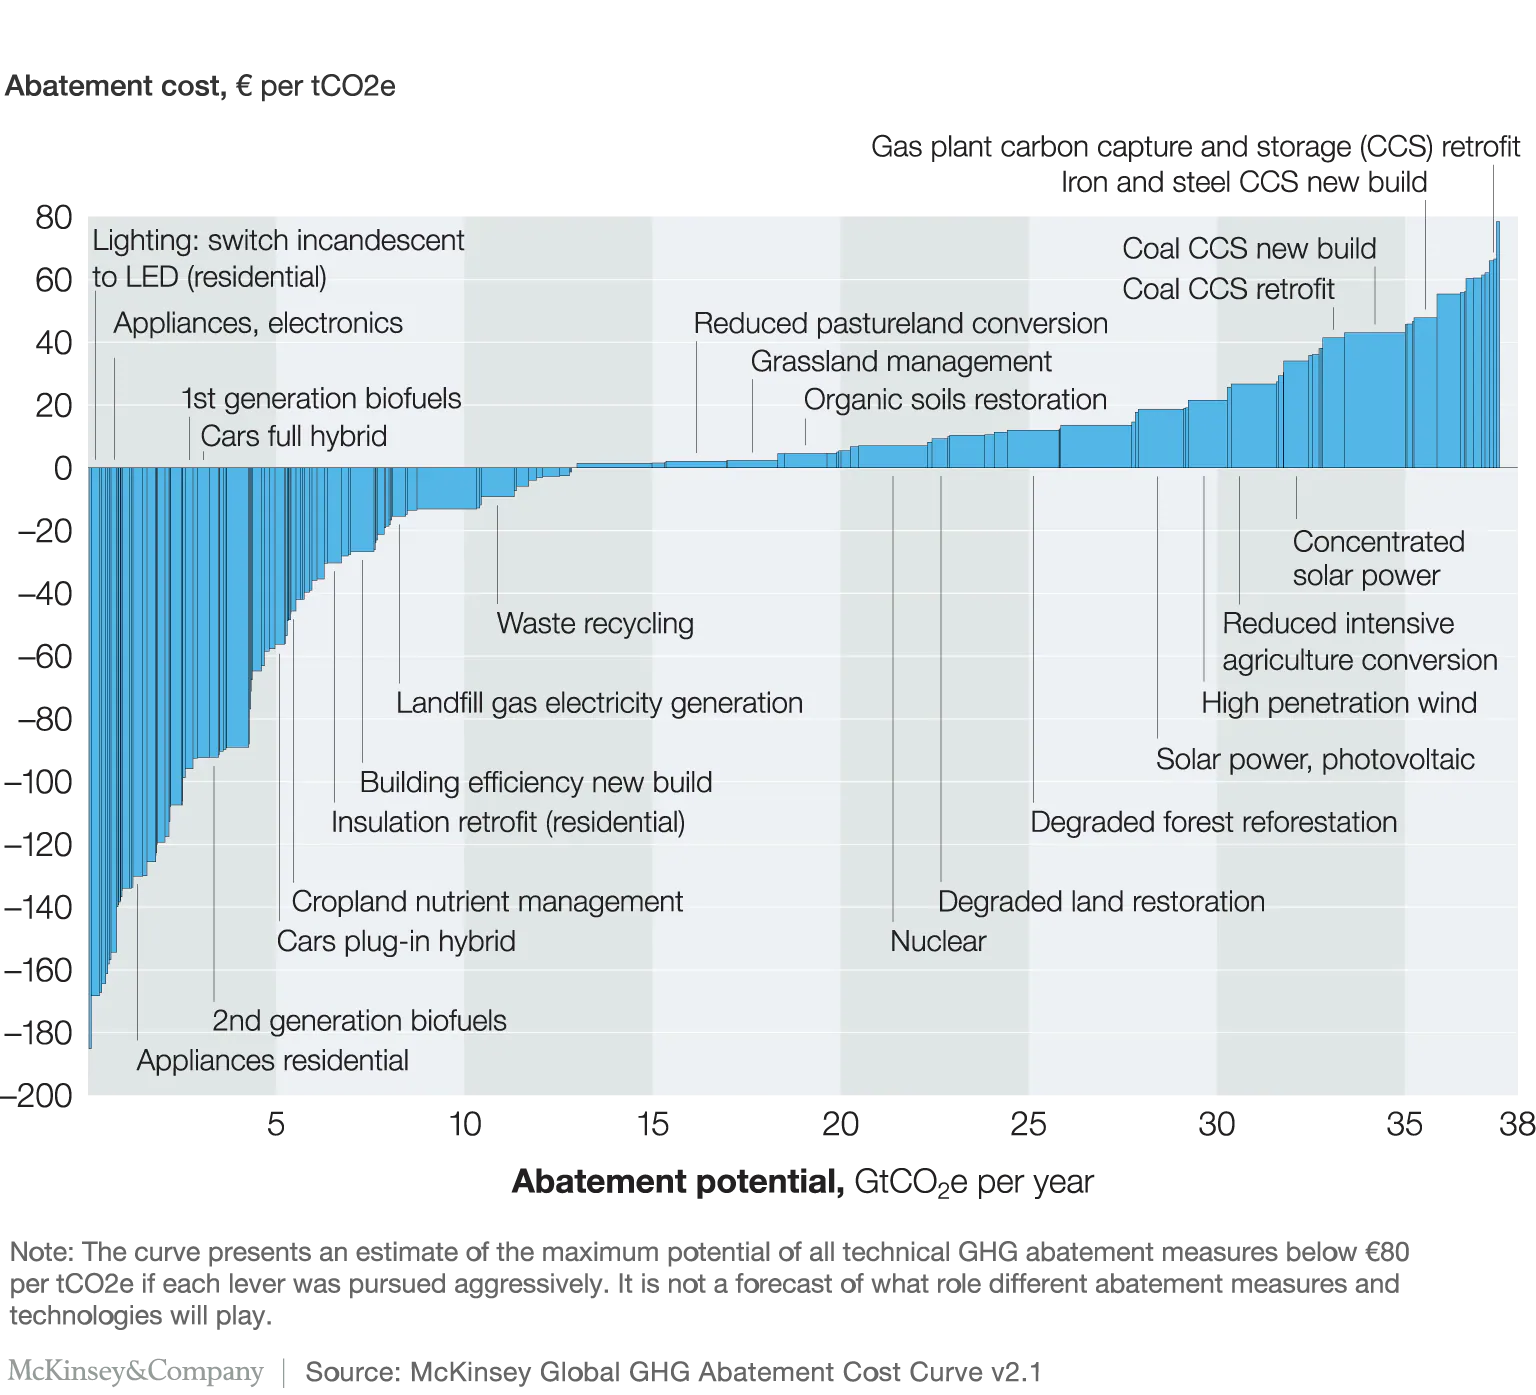
\includegraphics[width=0.8\textwidth]{figures/marginal_abatement_cost_curve.png}
\caption{Marginal Abatement Cost Curve. Adopted From \cite{McKinsey2017}}
\label{fig:macc}
\end{figure}
\noindent As we can observe from the graph, the MACC is upward-sloping, on the x-axis we have the quantity of emissions abated, and on the y-axis, we have the cost of abating one additional unit of emissions. Different industries and sectors will have different MACCs, and the shape of the MACC will depend on the cost of abatement measures and the quantity of emissions abated.

% \section{Financial Predictors Full-Size Graphs}
% \label{sec:FinancialPreds}

% \begin{figure}[H]
% \centering
% \subcaptionbox{Total Assets\label{fig:total-assets}}{%
%   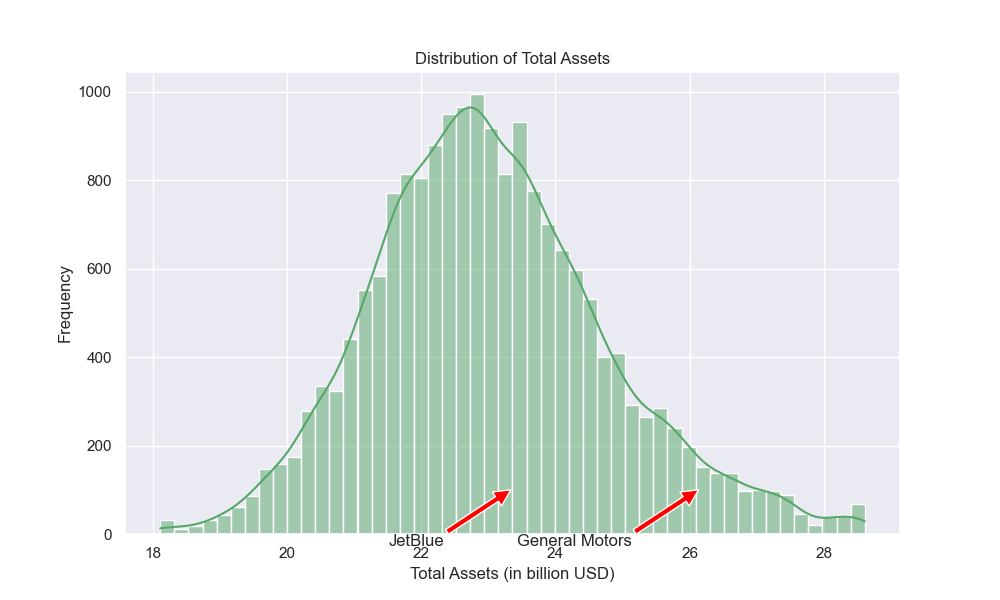
\includegraphics[width=0.8\textwidth]{figures/financial_preds/tot_assets_dist.png}}
% \caption{Financial Predictors: Total Assets}
% \end{figure}

% \begin{figure}[H]
% \centering
% \subcaptionbox{Market Capitalization\label{fig:market-capitalization}}{%
%   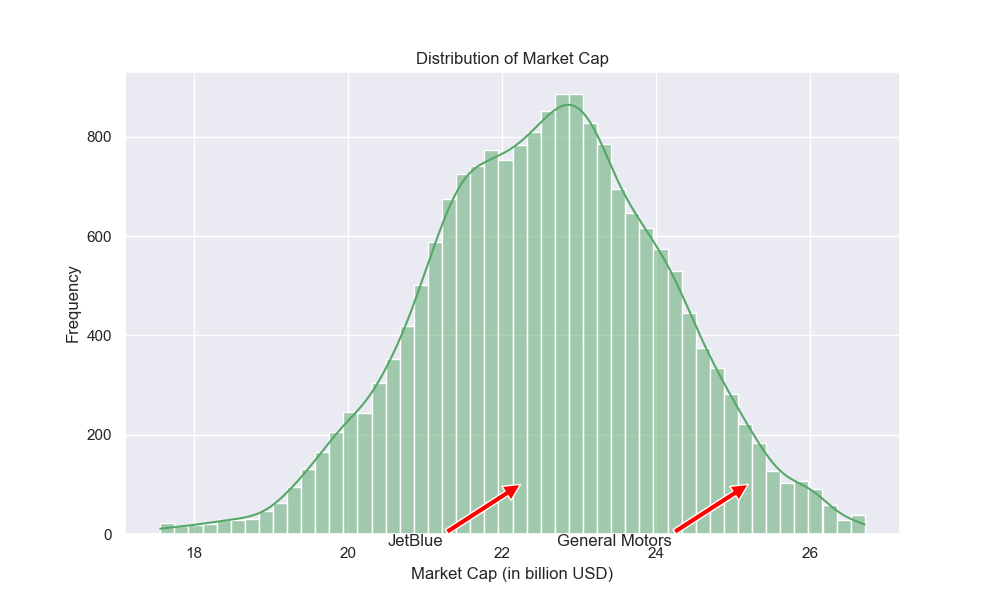
\includegraphics[width=0.8\textwidth]{figures/financial_preds/mkt_cap_dist.png}}
% \caption{Financial Predictors: Market Capitalization}
% \end{figure}

% \begin{figure}[H]
% \centering
% \subcaptionbox{Return on Equity\label{fig:roe}}{%
%   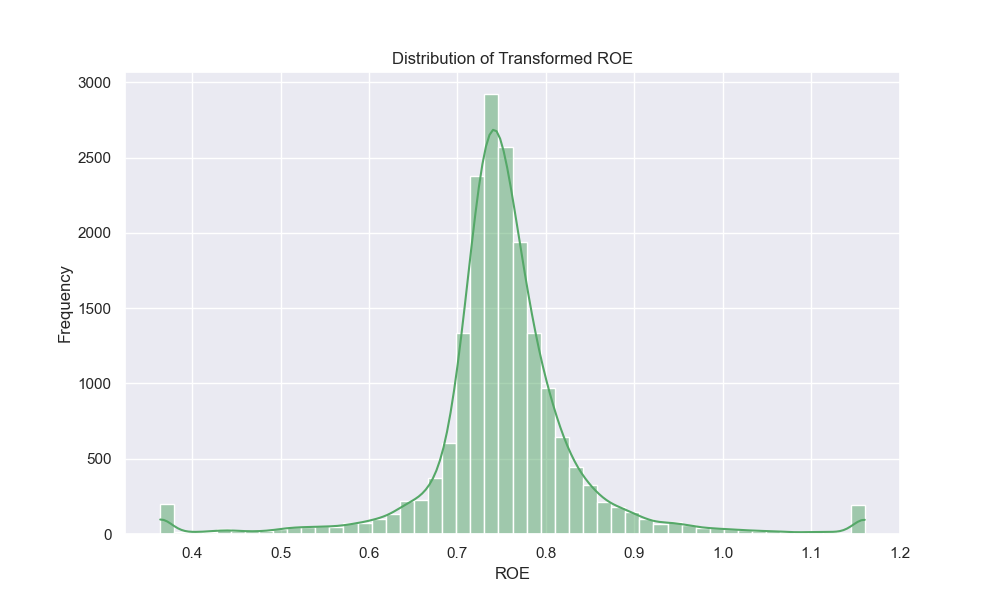
\includegraphics[width=0.8\textwidth]{figures/financial_preds/roe_dist.png}}
% \caption{Financial Predictors: Return on Equity}
% \end{figure}

% \begin{figure}[H]
% \centering
% \subcaptionbox{Revenue\label{fig:revenue}}{%
%   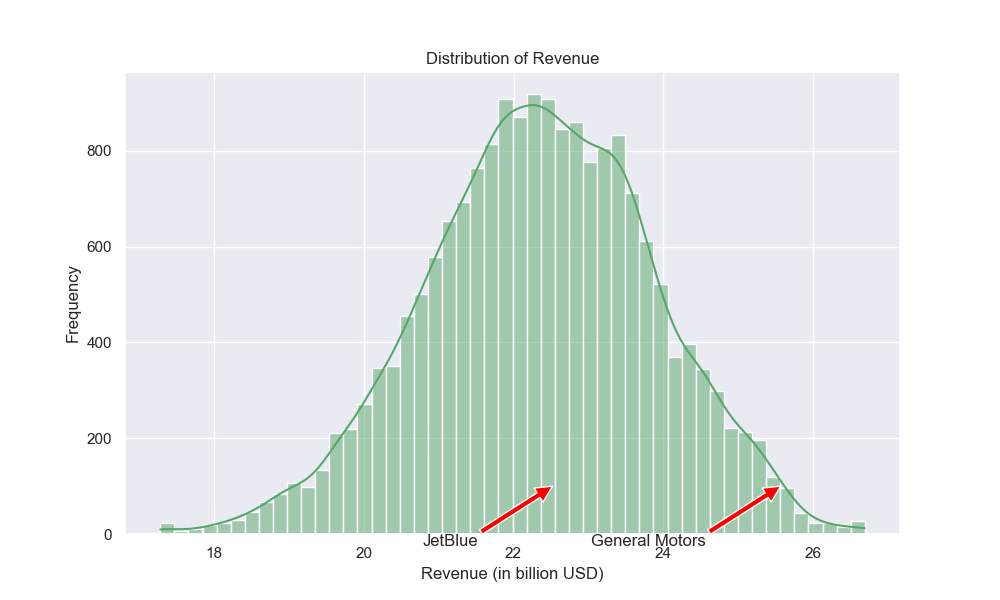
\includegraphics[width=0.8\textwidth]{figures/financial_preds/revenue_dist.png}}
% \caption{Financial Predictors: Revenue}
% \end{figure}

% \begin{figure}[H]
% \centering
% \subcaptionbox{Net Income\label{fig:net-income}}{%
%   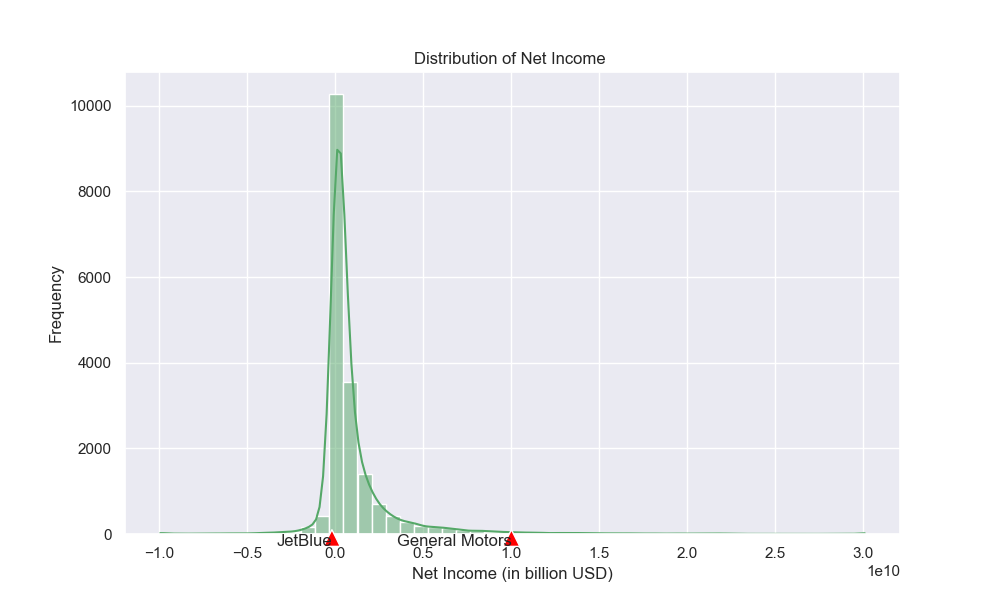
\includegraphics[width=0.8\textwidth]{figures/financial_preds/net_income_dist.png}}
% \caption{Financial Predictors: Net Income}
% \end{figure}

% \begin{figure}[H]
% \centering
% \subcaptionbox{Employees\label{fig:employees}}{%
%   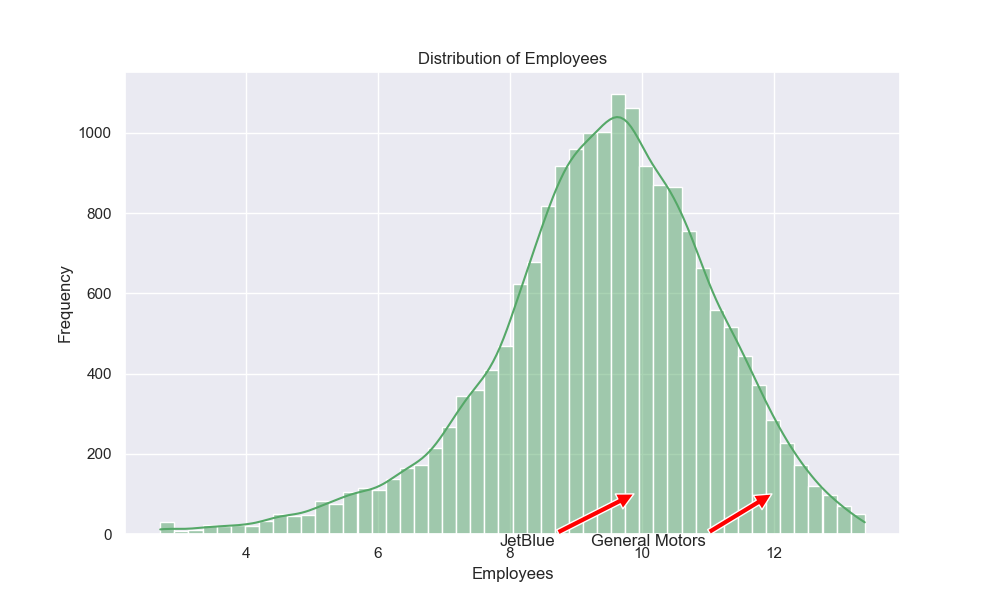
\includegraphics[width=0.8\textwidth]{figures/financial_preds/employees_dist.png}}
% \caption{Financial Predictors: Employees}
% \end{figure}

% \begin{figure}[H]
% \centering
% \subcaptionbox{Total Assets 1yr Growth\label{fig:total-assets-1yr-growth}}{%
%   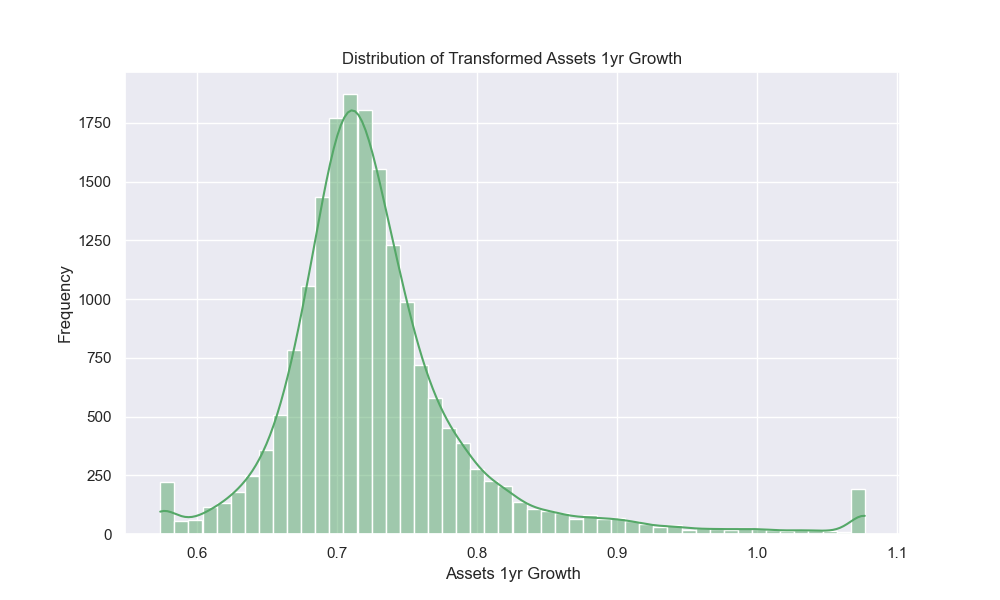
\includegraphics[width=0.8\textwidth]{figures/financial_preds/assets_1yr_growth_dist.png}}
% \caption{Financial Predictors: Total Assets 1yr Growth}
% \end{figure}

% \begin{figure}[H]
% \centering
% \subcaptionbox{Employees 1yr Growth\label{fig:employees-1yr-growth}}{%
%   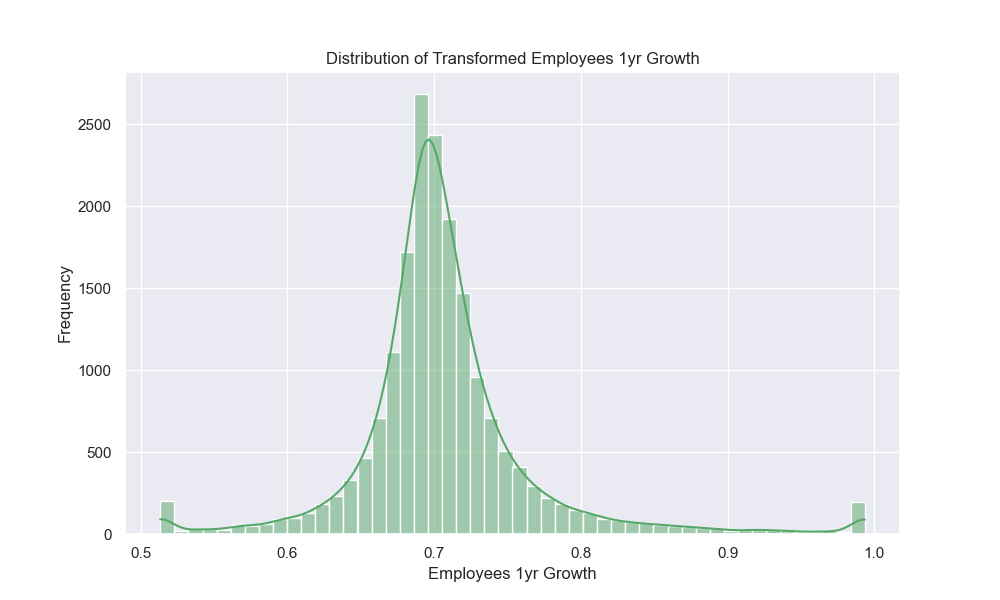
\includegraphics[width=0.8\textwidth]{figures/financial_preds/employees_1yr_growth_dist.png}}
% \caption{Financial Predictors: Employees 1yr Growth}
% \end{figure}

% \begin{figure}[H]
% \centering
% \subcaptionbox{Net Income Over Assets\label{fig:net-income-over-assets}}{%
%   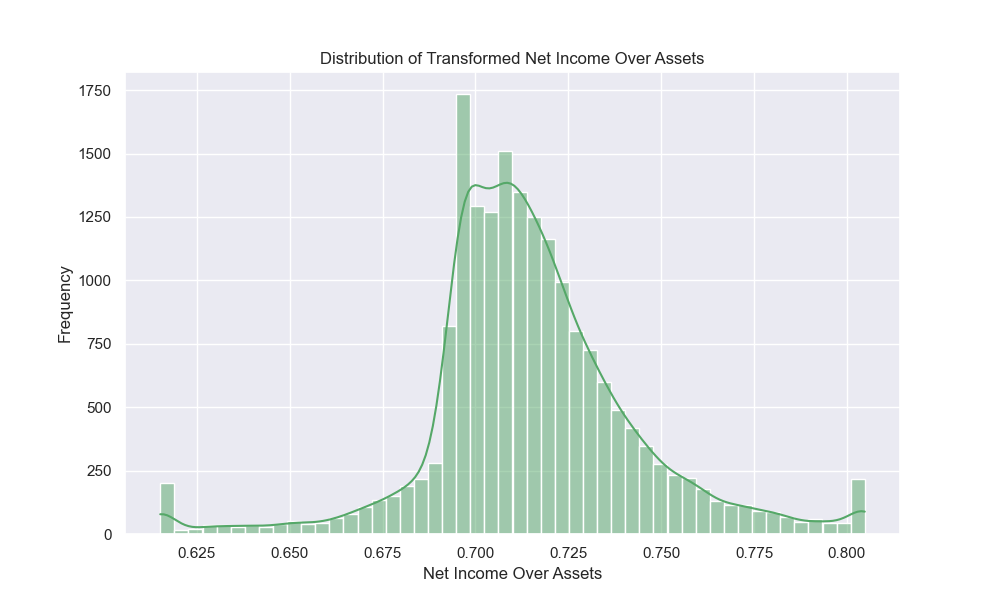
\includegraphics[width=0.8\textwidth]{figures/financial_preds/net_income_over_assets_dist.png}}
% \caption{Financial Predictors: Net Income Over Assets}
% \end{figure}


%  \setlength{\tabcolsep}{4pt}
%  \renewcommand{\arraystretch}{2.4}
% \footnotesize
% \begin{center}
%   \begin{tabular}{lcccc}
%     \hline
%  \textbf{Name} & \textbf{Param.} & \textbf{PMF or PDF} & \textbf{Mean} & \textbf{Variance} \\ 
%     \hline
%     Bernoulli & $p$ & $P(X=1) =p, P(X=0) = q$ & $p$ & $pq$ \\ 
%     Binomial & $n,p$ & ${n \choose k} p^k q^{n-k},   \,k \in \{0,1,\dots,n\}$ & $np$ & $npq$\\ 
%     FS & $p$ & $pq^{k-1},  \,k \in \{1,2,\dots\}$& $1/p$ & $q/p^2$\\ 
%     Geom & $p$ & $pq^{k},   \,k \in \{0,1,2,\dots\}$& $q/p$ & $q/p^2$\\ 
%     NBin & $r, p$ &  ${r+k-1 \choose r-1} p^r q^{k},  \,k \in \{0,1,2,\dots\}$ & $rq/p$ & $rq/p^2$ \\ 
%      HGeom & $w,b,n$ & $\frac{{w \choose k}{b \choose n-k}}{{{w+b} \choose n}}, \,k \in \{0,1,\dots,n\}$ & $\mu = \frac{nw}{w+b}$ & $(\frac{w+b-n}{w+b-1}) \mu (1-\frac{\mu}{n})$\\
%       NHGeom & $w,b,r$ & $ \frac{{r+k-1 \choose {r-1}}{w+b-r-k \choose w-r}}{{ {w+b} \choose {w}}},  \, k \in \{0,1,\dots,b\}$ & $\frac{rb}{w+1}$ & $ \frac{rb(w+b+1)(w-r+1)}{(w+1)^2(w+2)}$\\
%     Poisson & $\lambda$ & $\frac{e^{-\lambda} \lambda^k}{k!},  \,k \in \{0,1,2,\dots\}$ & $\lambda$ & $\lambda$ \\ 
%     Uniform & $a < b$ & $\frac{1}{b-a},   \,x \in (a,b)$ & $\frac{a+b}{2}$& $\frac{(b-a)^2}{12}$ \\ 
%     Normal & $\mu, \sigma^2$ & $\frac{1}{\sigma \sqrt{2\pi}}e^{-(x - \mu)^2/(2\sigma^2)}$ & $\mu$ & $\sigma^2$ \\ 
%     Log-Normal  &  $\mu, \sigma^2$ & $\frac{1}{x\sigma \sqrt{2\pi}}e^{-(\log x - \mu)^2/(2\sigma^2)},\, x > 0$ & $\theta = e^{ \mu + \sigma^2/2}$ & $\theta^2 (e^{\sigma^2} - 1)$\\
%     Expo & $\lambda$ &  $\lambda e^{-\lambda x}, \,x > 0$& $1/\lambda$ & $1/\lambda^2$ \\ 
%         Weibull & $\lambda, \gamma$ &  $ \gamma \lambda e^{-\lambda x^\gamma} x^{\gamma -1},  \,x > 0$& $\mu = \frac{\Gamma\left(1+1/\gamma \right)}{\lambda^{1/\gamma}}$ & $\frac{\Gamma\left(1 + 2/\gamma \right)}{\lambda^{2/\gamma}} - \mu^2$ \\ 
%     Gamma & $a, \lambda$ &  $\Gamma(a)^{-1} (\lambda x)^a e^{-\lambda x} x^{-1},  \,x > 0$& $a/\lambda$ & $a/\lambda^2$ \\ 
%     Beta & $a, b $ & $\frac{\Gamma(a + b)}{\Gamma(a)\Gamma(b)} x^{a-1}(1-x)^{b-1}, \,0<x<1$ & $\mu = \frac{a}{a+b}$ & $\frac{\mu (1-\mu)}{a+b+1}$\\
%    Chi-Square & $n$ & $\frac{1}{2^{n/2}\Gamma(n/2)}x^{n/2-1}e^{-x/2},  \,x>0$ & $n$ & $2n$\\
%     Student-$t$ & $n$ & $\frac{\Gamma((n+1)/2)}{\sqrt{n\pi} \Gamma(n/2)} (1+x^2/n)^{-(n+1)/2}$ & 0 if $n>1$ & $\frac{n}{n-2}$ if $n>2$\\
%     \hline
%   \end{tabular}
% \end{center}
% \normalsize

\section{Neural Network Model}

\subsection{Model Architecture}
\begin{figure}[H]
    \centering
    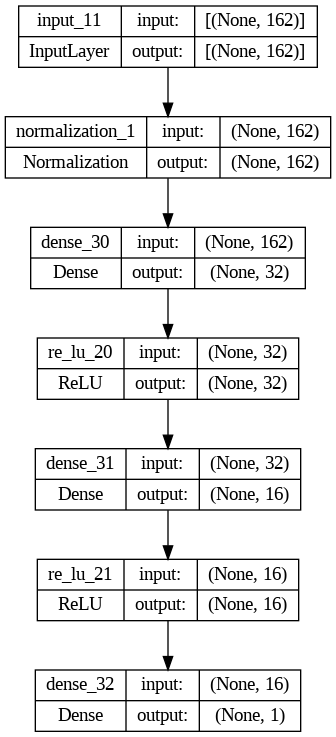
\includegraphics[width=0.4\textwidth]{figures/nn_architecture.png}
    \caption{Neural Networks Model Architecture}
    \label{fig:neural_networks_architecture}
\end{figure}

In this section I am reporting the configuration and the training and test results of a Neural Network model that was tested on the dataset. As can be observed from the performance metrics in Table \ref{tab:neural_networks_performance}, the model is in line with Mixed Effects regression and slightly worse than CatBoost. Given that it is less interpretable than other models, and because of the data considerations detailed previously, I believe that the questions tackled in this thesis do not benefit from Deep Learning techniques. Tree-based and parametric approach are preferable.

\subsection{Training and Validation Loss Plot}

\begin{figure}[H]
    \centering
    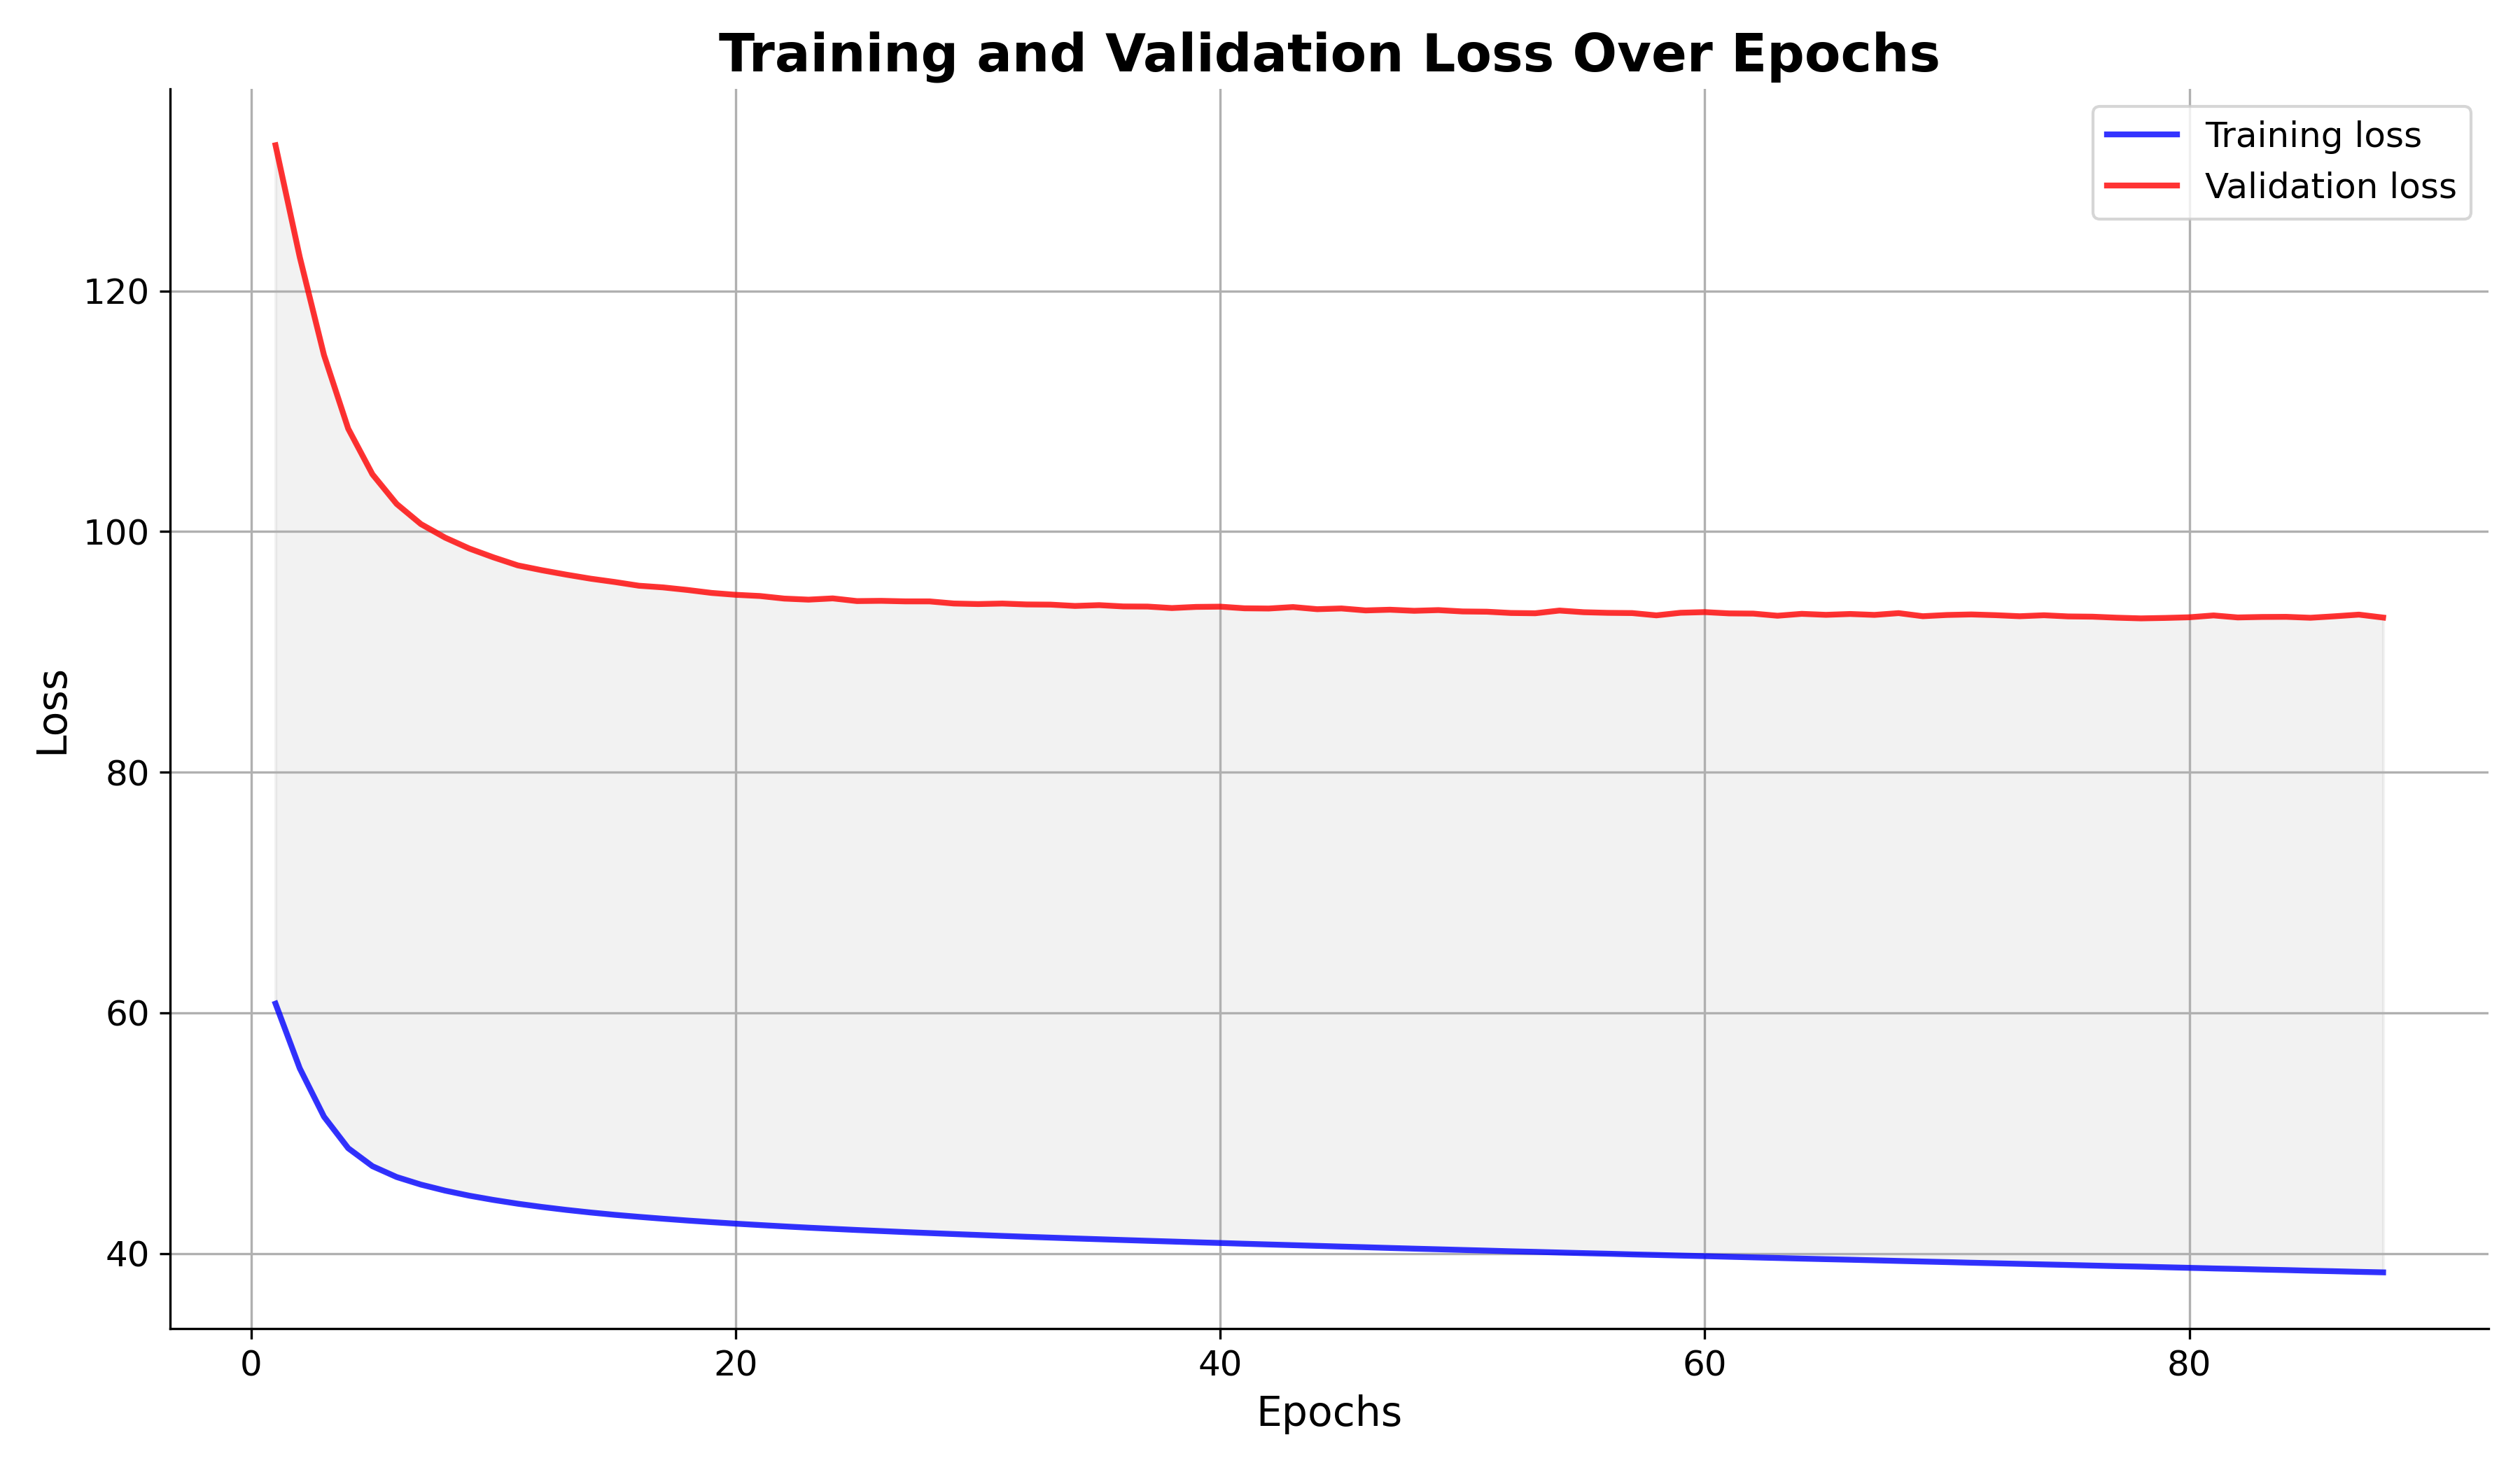
\includegraphics[width=0.8\textwidth]{figures/nn_training_loss.png}
    \caption{Neural Networks Model Training and Validation Loss Plot}
    \label{fig:neural_networks_loss_plot}
\end{figure}


\subsection{Model Performance Metrics}

\begin{table}[H]
    \centering
    \caption{Neural Networks Model Performance Metrics}
    \label{tab:neural_networks_performance}
    \begin{tabular}{lcccc}
    \hline
    Set & $R^2$ & RMSE & MSE & MAE \\ 
    \hline
    Training & 0.21 & 6.23 & 38.79 & 3.77 \\
    Test & 0.09 & 9.65 & 93.26 & 6.32 \\
    \hline
    \end{tabular}

\end{table}

\section{Variable Dictionary}
\label{sec:variable-dictionary}

\noindent Table~\ref{tab:variable-dictionary} provides an overview of the predictors used in the analysis, including their type, description, and source. Predictors are divided into three primary categories: \begin{itemize}
    \item \textbf{Firm Information:} Variables that describe the firm's characteristics, such as its unique identifier, reporting year, headquarters country, headquarters continent, and industry sector.
    \item \textbf{Financial Predictors:} Variables that capture the firm's financial performance, including total revenue, total assets, total employees, net income, and market capitalization.
    \item \textbf{CDP Predictors:} Variables derived from the CDP Climate Survey, such as the firm's emissions, energy consumption, and climate-related targets and initiatives.
\end{itemize}


\begin{longtable}{lp{1cm}p{6cm}p{1.1cm}} \\
    \toprule
    \textbf{Variable} & \textbf{Type} & \textbf{Description} & \textbf{Source} \\
    \midrule
    \endfirsthead % Everything above goes at the top of the first page of the table
    \multicolumn{4}{c}%
    {\tablename\ \thetable\ -- \textit{Continued from previous page}} \\
    \toprule
    \textbf{Variable} & \textbf{Type} & \textbf{Description} & \textbf{Source} \\
    \midrule
    \endhead % Header to be repeated on every page
    \bottomrule
    \multicolumn{4}{r}{\textit{Continued on next page}} \\
    \endfoot % Footer to be repeated on every page except the last
    \endlastfoot % Footer for the last page of the table
    
    % Core Information Section
    \multicolumn{4}{l}{\textbf{Firm Information}} \\
    \midrule
    ID & cat & unique firm identifier & CDP \\
    Year & num & reporting year & CDP \\
    Country & cat & headquarters country  & CDP \\
    Continent & cat & headquarters continent derived from country & CDP \\
    Industry & cat & Global Industry Classification Standard 25 industry sectors & GICS \\
    
    \midrule
    % Financial Predictors Section
    \multicolumn{4}{l}{\textbf{Financial Predictors}} \\
    \midrule
    log(Revenue) & num & natural logarithm of total revenue & WS \\
    log(Assets) & num & natural logarithm of total assets & WS \\
    log(Assets 1yr gr.) & num & natural logarithm of total assets growth & WS \\
    log(Employees) & num & natural logarithm of total employees & WS \\
    log(Empl. 1y gr.) & num & natural logarithm of total employees growth & WS \\
    log(Net Income) & num & natural logarithm of net income & WS \\
    log(Market Cap) & num & market capitalization & WS \\
    log(Roe) & num & natural logarithm of return on equity & WS \\
    log(Revenue) & num & natural logarithm of total revenue & WS \\
    % Add more variables as needed
    \midrule
    % CDP Predictors Section
    \multicolumn{4}{l}{\textbf{CDP Predictors}} \\
    \midrule
    Ghg.Change.Real.Next & num & Change in real GHG emissions from previous year & CDP  \\
    Proportion.Verified.Scope1 & num & Proportion of Scope 1 GHG emissions that are verified & CDP  \\
    Ghg1 & num & Total direct (Scope 1) GHG emissions & CDP  \\
    Ghg2Location & num & Location-based Scope 2 GHG emissions & CDP  \\
    Ghg2Market & num & Market-based Scope 2 GHG emissions & CDP  \\
    Ghg3.Total & num & Total Scope 3 GHG emissions & CDP  \\
    Ghg3.Count & num & Count of Scope 3 GHG emissions sources reported & CDP  \\
    Ghg1.Na & cat & Indicator if Scope 1 GHG data is not available & CDP  \\
    Ghg2Location.Na & cat & Indicator if location-based Scope 2 data is not available & CDP  \\
    Ghg2Market.Na & cat & Indicator if market-based Scope 2 data is not available & CDP  \\
    Ghg3.Total.Na & cat & Indicator if Scope 3 data is not available & CDP  \\
    Methane.Emissions & num & Total methane GHG emissions & CDP  \\
    Type.Scope1 & cat & Type of Scope 1 emissions verification & CDP \\
    Ghg.Verification.Scope1.Yes & cat & Indicator if Scope 1 emissions are verified & CDP \\
    Ghg.Verification.Scope2.Yes & cat & Indicator if Scope 2 emissions are verified & CDP \\
    Ghg.Verification.Scope3.Yes & cat & Indicator if Scope 3 emissions are verified & CDP \\
    Method.Ind & cat & Indicator of the incentive method used & CDP \\
    Cdp.Boardoversight.I & num & Board oversight on climate-related issues & CDP \\
    Cdp.Incentivebinary.I & cat & Presence of incentives for climate-related performance & CDP \\
    Cdp.Baseyearemission.Mean & num & Average of baseline year emissions data & CDP \\
    Cdp.Targetscope.Mean & num & Average percentage of emissions scopes covered by targets & CDP \\
    Cdp.Targetamount.Mean & num & Mean target emission reduction amount & CDP \\
    Cdp.Targettype.Absolute & cat & Presence of absolute emission reduction targets & CDP \\
    Cdp.Targettype.Intensity & cat & Presence of intensity-based emission reduction targets & CDP \\
    Cdp.Aggregated.Risk & num & Aggregated measure of climate-related risks & CDP \\
    Cdp.Aggregated.Opp & num & Aggregated measure of climate-related opportunities & CDP \\
    Initiative.Scope1 & cat & Initiative related to Scope 1 emissions & CDP \\
    Initiative.Scope2 & cat & Initiative related to Scope 2 emissions & CDP \\
    Initiative.Scope3 & cat & Initiative related to Scope 3 emissions & CDP \\
    Absent.Cdp.Initiative & cat & Indicator if firm-year data is absent in CDP initiative processed CSV & CDP \\
    Co2.Counter & num & Count of CO2 reduction initiatives & CDP \\
    Msaving.Counter & num & Count of money-saving initiatives due to emission reductions & CDP \\
    Investment.Counter & num & Number of investments in emission reduction initiatives & CDP \\
    Investment.Total.Log1P & num & Log-transformed total investment in emission reduction (log1p) & CDP \\
    Cdp.Num.Credits.Clean.Count & num & Count of clean energy credits & CDP \\
    Clean.Credit.Origination & cat & Origin of clean energy credits (original or purchased) & CDP \\
    Cdp.PurposeVoluntary.Offsetting & cat & Purpose of clean energy credits for voluntary offsetting & CDP \\
    Absent.Cdp.Carbon.Credits & cat & Indicator if carbon credits data is absent in processed CSV & CDP \\
    % Add more variables as needed
    \bottomrule
\caption{Variable Dictionary}
\label{tab:variable-dictionary}
\end{longtable}

\section{A Case Study on Two CDP Reports}

In this section, I will analyze the  2022 CDP reports from: General Motors (GM) in the automotive sector and Jet Blue in the airline industry. They are obtained as part of CDP data, and can the full reports in PDF form can be requested through the CDP website \cite{Cdp2017}. These reports are examples of the highly company-specific nature of emission data, with significant variances deriving from the fact that the companies operate in different sectors. Through this exploration, we therefore uncover a primary challenge for data analysis on the CDP Survey: there is a significant amount of text-based and free-form answers within the CDP reports.

\subsection{General Motors 2022 CDP Report}
General Motors Company (GM), a global leader in the automotive industry, is headquartered in Detroit, Michigan, USA. Renowned for its ownership and production of the Chevrolet, GMC, Cadillac, and Buick brands, GM was the largest automaker in the United States by sales in 2022 \cite{GeneralMotorsWikipedia}. GM's commitment to sustainability is evident in its comprehensive governance and ambitious environmental targets.

\subsection*{Scope 1 and Scope 2 Emissions}
GM has set forth aggressive targets to reduce its Scope 1 and Scope 2 emissions by 71.4\% by 2035, relative to its 2018 baseline. In 2018, GM reported Scope 1 emissions of 1,763,555 metric tons CO2e and Scope 2 emissions of 3,924,338 metric tons CO2e. By the reporting year 2022, GM achieved a reduction to 1,252,906 metric tons CO2e for Scope 1 and 2,150,694 metric tons CO2e for Scope 2, marking significant progress towards its goal. This reduction aligns with the 1.5 degrees Celsius strategy set by the Paris Agreement, underscoring GM's commitment to global climate initiatives \cite{GeneralMotorsWikipedia, Zhou2020Decarbonization}.

GM's strategy includes enhancing energy efficiency across its manufacturing operations and increasing the use of renewable energy. In 2021, GM implemented over 300 energy efficiency improvements, such as upgrading to more efficient equipment and increasing renewable electricity use from 23\% to 25\%, contributing to GHG reductions in Scope 2 emissions.

\subsection*{Scope 3 Emissions}
Addressing Scope 3 emissions, GM has set a target to achieve a 50.4\% reduction in its vehicle use emissions, from a baseline of 0.0002466 metric tons of CO2 per kilometer to 0.0001223136. GM's strategy to meet this target includes transitioning to an all-electric vehicle (EV) future, with plans to introduce 30 new EV models by 2025 and aspirations to be fully electric by 2035. Partnerships to increase renewable energy generation and deploy EV chargers, in collaboration with EvGo, are examples of GM's intent of reducing its carbon footprint across the value chain, thus addressing Scope 3 figures.
 
\subsection*{Key Takeaways}
\begin{itemize}
    \item \textbf{Emissions Reduction Track Record:} GM's targeted reductions in Scope 1 and Scope 2 emissions are examples of a concrete commitment to environmental stewardship, leveraging technological advancements and renewable energy.
    \item \textbf{Electric Vehicles:} GM's aggressive transition to an all-EV lineup by 2035 highlights its leadership role in transforming the automotive industry and promoting decarbonization
    \item \textbf{Comprehensive Approach to Sustainability:} Through its Scope 3 emissions reduction target, GM also addresses the broader environmental impact of its products, emphasizing the importance of a decarbonization strategy that goes beyond direct emissions.
\end{itemize}

Overall, GM's sustainability efforts are examples of a strong commitment to reducing environmental impact and showcasing a concrete path towards decarbonizing. Note how this requires profound changes in technology to GM's fleet which represent major challenges. Thus, although there is a concrete path, there is uncertainty on whether GM will be able to deliver on all its decarbonization commitments. 


% \subsection{General Motors' Report Analysis}

% \noindent General Motors Company (GM), an American multinational automotive manufacturing giant, is headquartered in Detroit, Michigan, USA. Esteemed for its ownership and production of four prominent automobile brands—Chevrolet, GMC, Cadillac, and Buick—it stood as the largest automaker in the United States by sales in 2022 \cite{GeneralMotorsWikipedia}. At the core of GM's corporate strategy lies a robust sustainability framework, spearheaded at the enterprise level. This framework encompasses oversight by the Board, the Chief Executive Officer, and the Chief Sustainability Officer, alongside a dedicated Board-level committee tasked with addressing climate-related challenges. Furthermore, the company has instituted a monetary incentive for its corporate executive team, primarily tethered to the deployment and success of its electric vehicle (EV) fleet.

% \noindent In pursuit of environmental sustainability, GM has set ambitious targets to reduce its Scope 1 and Scope 2 emissions by 71.4\% by 2035, relative to its 2018 baseline, where emissions were recorded at 1,763,555 and 3,924,338 metric tons CO2e for Scope 1 and Scope 2, respectively. As of 2022, the company has realized 56.24\% of this target, with reported emissions of 1,252,906 for Scope 1 and 2,150,694 for Scope 2, aligning with the 1.5 degrees Celsius strategy of the Paris Agreement \cite{Zhou2020Decarbonization}. GM's progress is attributed to enhanced energy efficiency in its manufacturing processes and a strategic shift towards renewable energy procurement.

% \noindent The company's sustainability report highlights the implementation of over 300 energy efficiency improvements in 2021 across its buildings and processes. These include the adoption of more efficient equipment, such as variable speed drives on motors, process controls, LED lighting, among other conservation measures. Additionally, GM increased its renewable electricity usage from 23\% to 25\%, further contributing to reductions in Scope 2 market-based emissions. This approach exemplifies how the automotive industry can effectively reduce emissions through renewable energy adoption and manufacturing efficiencies, a stark contrast to sectors like cement production, which accounts for 7\% of global anthropogenic greenhouse gas emissions and faces significant decarbonization challenges due to the inherent CO2 generation during limestone calcination \cite{Ostovari2021}.

% \noindent However, the most daunting challenge for GM lies within Scope 3 emissions, predominantly stemming from vehicle use and fossil fuel combustion. While the company has not provided an estimate for its Scope 3 emissions, it aims to reduce these emissions by 50.4\% from a baseline of 0.0002466 metric tons of CO2 per kilometer to 0.0001223136. Achieving this reduction is contingent upon GM's strategic pivot to an all-EV future, underscored by its commitment to launch 30 new EV models by 2025, transition entirely to EVs by 2035, and bolster renewable energy generation and EV charger deployment in collaboration with EvGo, a leading charging network, with an aim to power these chargers entirely by renewable energy. This strategy underscores the critical insights for the automotive industry:
% \begin{itemize}
%     \item Scope 3 emissions, primarily from vehicle use, constitute the most significant share of emissions, presenting the greatest reduction challenge.
%     \item GM is actively enhancing its production processes and renewable energy initiatives, demonstrating tangible success in emission reduction efforts.
%     \item The reduction of Scope 3 emissions hinges on a more complex strategy, currently in its nascent stages, with GM having achieved only 0.225\% progress toward its target, underscoring the enormity of the challenge ahead.
% \end{itemize}

\subsection{JetBlue Airways Corporation 2022 CDP Report}
JetBlue Airways Corporation is  focusing on reducing Scope 1, Scope 2, and Scope 3 emissions across its operations. The airline's governance structure emphasizes sustainability, with strategic initiatives overseen by its board and executive team.

\subsection*{Scope 1 and Scope 2 Emissions}
In the reporting year 2022, JetBlue's Scope 1 emissions totaled 6,853,927 metric tons CO2e, predominantly from jet fuel combustion, the main source of emissions within the airline industry. Scope 2 emissions amounted to 25,945 metric tons CO2e, reflecting the emissions from electricity consumption. These figures demonstrate JetBlue's significant environmental footprint which is typical of a firm in the airline industry. Again here, we can observe how technology is a crucial factor in determining the composition of a firm's emission.

JetBlue's strategies to mitigate these carbon figures include modernizing its fleet with more fuel-efficient aircraft, such as the Airbus A220 and A321Neo, and investing in sustainable aviation fuel (SAF) to reduce lifecycle GHG emissions associated with jet fuel. Additionally, the airline is transitioning its ground service equipment to electric power, this is in line with its commitment to lower Scope 1 and Scope 2 emissions.

\subsection*{Scope 3 Emissions}
JetBlue's Scope 3 emissions are an important component of its sustainability strategy as well, with the airline currently monitoring emissions from purchased goods and services, capital goods, and fuel-and-energy-related activities not included in Scope 1 or 2. In 2022, the emissions reported were as follows:

\begin{itemize}
    \item Purchased Goods and Services: 44,922 metric tons CO2e, estimated for catered food and onboard product.
    \item Capital Goods: 485,629 metric tons CO2e, associated with aircraft ground equipment and spare parts.
    \item Fuel-and-Energy-Related Activities: 1,391,126 metric tons CO2e, highlighting the broader impact of JetBlue's operational energy use.
\end{itemize}

These figures were calculated using the Quantis Scope 3 tool. Overall, the airline's commitment to understanding and reducing its Scope 3 emissions is evident through its detailed reporting and targeted reduction strategies, including investments in SAF and efficiency improvements across its value chain.

\subsection*{Key Takeaways}
\begin{itemize}
    \item \textbf{Comprehensive Emission Reduction:} JetBlue's efforts to reduce Scope 1, Scope 2, and Scope 3 emissions underscore a comprehensive approach to sustainability, addressing both direct and indirect sources.
    \item \textbf{Innovation and Efficiency:} Through fleet modernization, SAF investments, and operational efficiencies, JetBlue is actively working towards reducing its environmental impact, despite the inherent challenges of the airline industry.
    \item \textbf{Scope 3 Emissions:} JetBlue's detailed reporting on Scope 3 emissions highlights the potential for using standardized tools, such as Quantis, to facilitate the measurement of indirect emissions.
\end{itemize}


\section{Code Repository}
\label{sec:code-repo}

The code repository for this thesis project is available on GitHub at the following link: \url{https://github.com/fabrisera/thesis_project}. The repository contains the code for data preprocessing, exploratory data analysis, feature engineering, model development, evaluation and the Tex files for the thesis document. I primarily used Python for data cleaning, EDA, and modeling. I also used R specifically for the Mixed Effect Models. The CDP data is not included in the repository due to confidentiality reasons, but the code is structured to work with the standard CSV and Excel files provided by the CDP. Thus, to replicate these results, it will be sufficient to obtain the data, clone the repository, and re-run all the scripts.